\chapter[Introduction]{Introduction}

\epigraph{I was born not knowing and have had only a little time to change that here and there.}
{\textit{Richard Feynman \\ Letter to Armando Garcia J.}}


\minitoc

\section{Motivation and context}

This work aims at exploring the port-Hamiltonian (pH) framework as a modelling paradigm, with particular emphasis for the case of flexible structures. This framework enjoys many interesting properties, since it intrinsically merges geometry with network theory \cite{vanderschaft2006book}. A powerful feature of this formalism, especially for the modelling task, is its modularity. Finite-dimensional port-Hamiltonian systems (pHs) can be easily interconnected together, as shown in \cite{cervera2007interconnection}. The interconnection is also possible in the infinite-dimensional case \cite{kurula2010}. Eventually, it is also possible to merge finite and infinite pH systems \cite{pasumarthy2006}. This features is especially useful to simplify the modelling task in preliminary analyses, or, conversely, to achieve high-fidelity models of complex multiphysics phenomena. Examples of multiphysics problems are brain edema simulations \cite{ju2020brain} (cf. Fig. \ref{fig:p_brain}) or plasma physics \cite{nattila2019runko} (cf. Fig. \ref{fig:plasma}). \\





\begin{figure}[htbp]%
	\centering
	\subfloat[][Normal brain]{%
		\label{fig:p_normal}%
		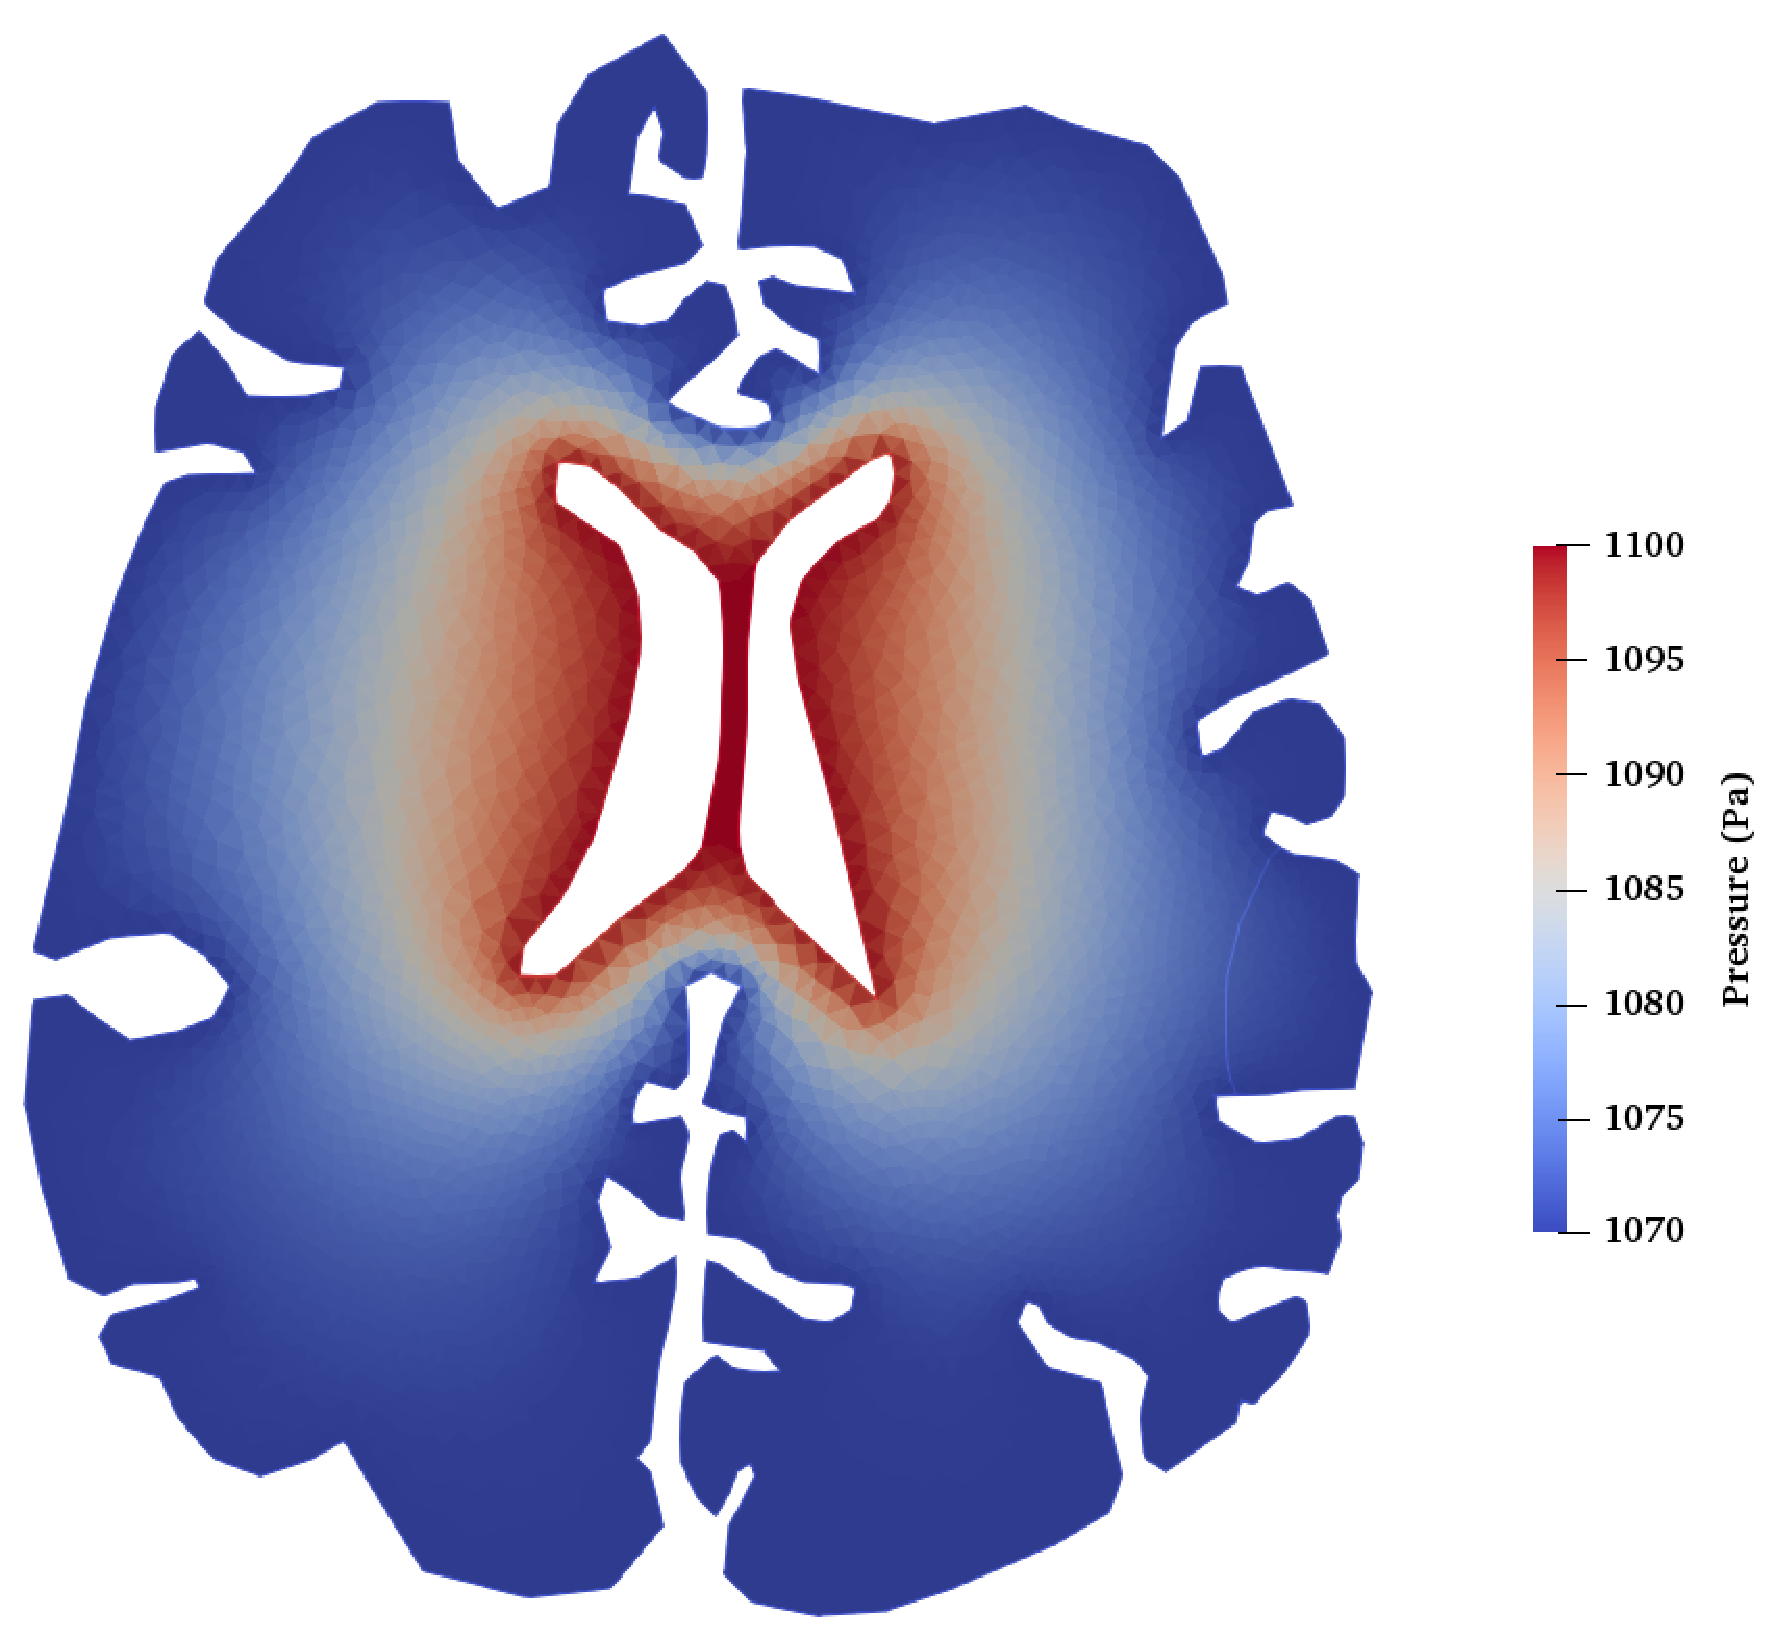
\includegraphics[width=0.48\columnwidth]{part_1/brain_normal_p.eps}} 
	\hspace{8pt}%
	\subfloat[][Injured brain]{%
		\label{fig:p_injured}%
		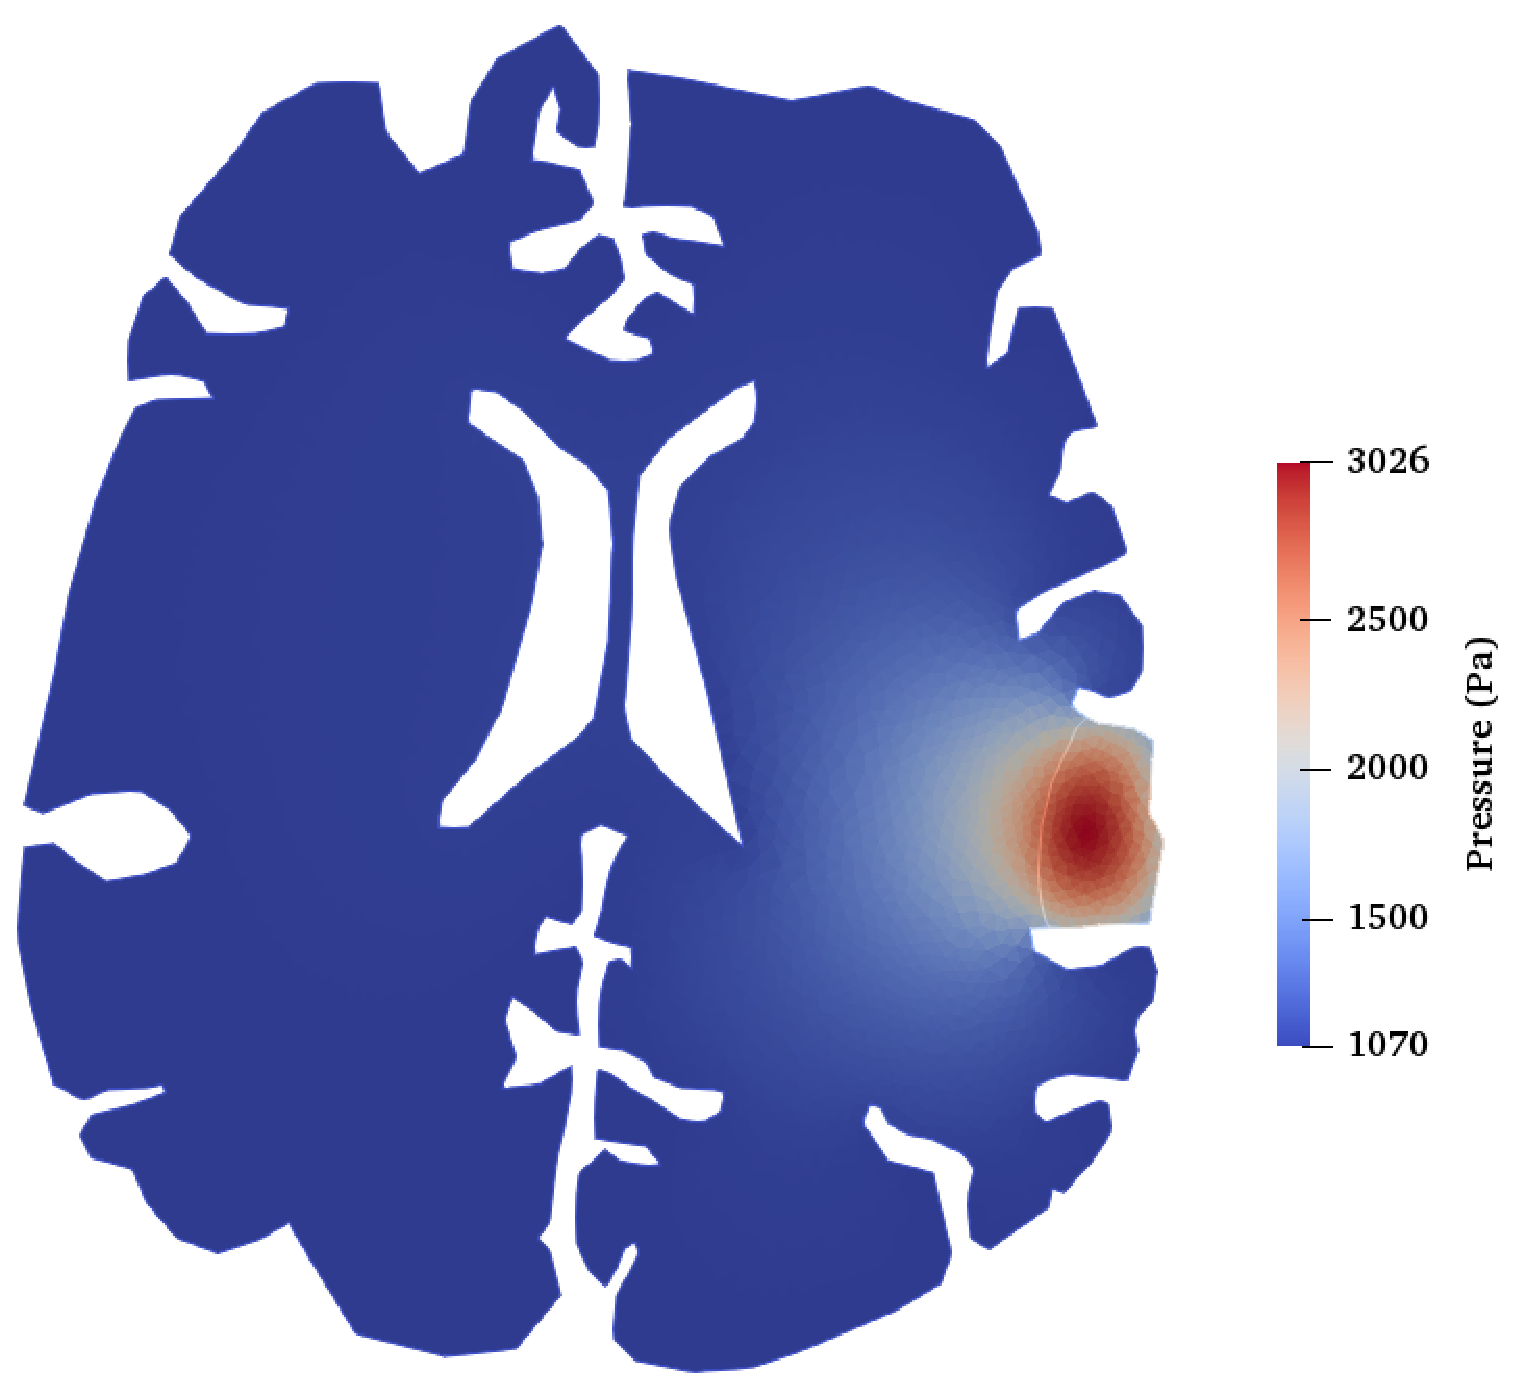
\includegraphics[width=0.48\columnwidth]{part_1/brain_injured_p.eps}}%
	\caption[]{From \cite{ju2020brain}, simulated pressure within the brain for a physiological (left) and injured (right) condition. The authors proposed a coupled multiphysics framework to solve the underlying Biot system. The discretization is achieved using mixed finite elements.}%
	\label{fig:p_brain}%
\end{figure}

\begin{figure}[htbp]%
	\centering
	\subfloat[][Plasma density]{%
		\label{fig:rho_plasma}%
		\includegraphics[width=0.48\columnwidth]{part_1/rho.pdf}}%
	\hspace{8pt}%
	\subfloat[][Out-of-plane plasma current density]{%
		\label{fig:jz_plasma}%
		\includegraphics[width=0.48\columnwidth]{part_1/jz.pdf}} 
	\caption[]{From \cite{nattila2019runko}, density field (left) and current density (right) for plasma kinetic turbulence simulations. The authors employs the Yee finite difference scheme \cite{yee1966numerical} to approximate the Vlasov-Maxwell equations and a full relativistic Boris scheme \cite{boris1970relativistic} to update the particles velocity and position.}%
	\label{fig:plasma}%
\end{figure}

\section{Literature review}
A brief literature review of the topics considered in the thesis is made here. This is by no means an exhaustive discussion. Throughout the chapters of the thesis, the literature is also referenced.


\subsection{Port-Hamiltonian distributed systems}
\textbf{Differential geometry}
An interesting reference that can provide some ideas in this direction is \cite{yao2011modeling,nishida2004}. 

For 1D linear PH systems with a generalized skew-adjoint system operator, \cite{legorrec2005} gives conditions on the assignment of boundary inputs and outputs for the system operator to generate a contraction semigroup. The latter is instrumental to show well-posedness of a linear PH system, see \cite{zwart2012}. Essentially, at most half the number of boundary port variables
can be imposed as control inputs for a well-posed PH system in one-dimensional domains. The complete characterization of pH in arbitrary dimension is still an open research field. Two notable exceptions \cite{zwart2015wave,skrepek2019wellposedness} provide partial answers to this problem. The first demonstrate the well-posedness of the linear wave equation in arbitrary geometrical dimensions. The second generalizes this result to treat the case of generic first order linear pHs in arbitrary geometrical dimensions. \\


\subsection{Structure-preserving discretization}

\subsection{Mixed finite element for elasticity}

Thanks to \cite{cardoso2018pfem}, it has become evident that there is a strict link between  discretization of port-Hamiltonian (pH) systems and mixed finite elements. Velocity-stress formulation for the wave dynamics and elastodynamics problems are indeed Hamiltonian and their mixed discretization preserves such a structure. For instance in \cite{kirby2015} the authors employed mixed finite elements to obtain a  symplectic semi-discretization for the wave equation. This allows using known finite element scheme to preserve the pH structure at the discrete level.

Mixed finite elements for the wave equation have been studied in \cite{geveci1988,becache2000wave}. For elastodynamics the construction of stable elements gets more complicated because of the presence of the symmetric stress tensor. Existing elements enforce symmetry either strongly \cite{becache2001elas} or weakly \cite{arnold2014elastodynamics}.

\subsection{Multibody dynamics}

In structural control co-design of flexible multibody systems, it is especially useful to dispose of a modular description, to simplify analysis. In this spirit, the transfer matrix method \cite{rong2010transfer} and the component mode synthesis \cite{hurty1965cms} are two well known substructuring techniques that allow the construction of complex multibody systems by interconnecting subcomponents together. A reformulation of the Finite Element-Transfer Matrix (FE-TM) method \cite{tan1990transfer} allows an easy construction of reduced models that are suited for decentralized control design. For the component mode synthesis, the controlled component synthesis (CCS), a framework for the design of decentralized controller of flexible structures, has been proposed in \cite{young1990}. Another modeling paradigm based on the component mode synthesis is the two-input two-output port (TITOP) approach \cite{alazard2015titop}. It conceives the dynamical model of each substructure as a transfer between the accelerations and the external forces at the connection points. This feature allows considering different boundary conditions by inverting specific channels in the transfer matrix. A rigorous validation was provided in \cite{perez2016flexible,sanfedino2018finite}, where the robustness of the methodology in handling various boundary conditions was assessed. \\
\indent The Lagrangian formulation is the most commonly used methodology to retrieve the equations of motion of flexible multibody systems. {Using the variational principles of geometric mechanics the equations of motion in Hamiltonian form can be derived either for rigid body dynamics \cite[Proposition 7.1.1]{holm2008geometric} and general non linear elasticity \cite[Chapter 3]{marsden1981lectures}.} The port-Hamiltonian (pH) framework \cite{duindam2009} has been recently employed to describe the dynamics of rigid and flexible links \cite{macchelli2007link,macchelli2009multi}. PH systems are intrinsically modular \cite{cervera2007interconnection}, hence this approach naturally allows constructing complex system by interconnecting together atomic elements. The formulation therein naturally accounts for the non-linearities due to large deformations.  However, this methodology relies on Lie algebra and differential geometry concepts and requires non standard discretization techniques \cite{golo2004hamiltonian}. Thus, the overall implementation is not straightforward. \\
\indent Together with the approach used to derive the equations of motion, the incorporation of the elastic motion represents another important point when dealing with flexible multibody systems. Three descriptions are commonly used: the floating frame formulation, the corotational frame formulation and the inertial frame formulation \cite{ellenbroek2018}. The choice greatly depends on the foreseen application.  The corotational and inertial frame formulations take into account large deformations of the elastic body, hence are well-suited for accurate simulations. {For these formulation many model reduction strategies have been developed in the last two decades \cite{rong2019}.} The inclusion of active control strategies is often unfeasible due to the computational burden \cite{wasfy2003survey}. The floating frame formulation is less accurate but easily integrates many model reduction techniques \cite{nowakowski2012}, making it possible to obtain a low-dimensional problem for control design. \\
\indent {The strong form Lagrangian formulation of flexible dynamics using a floating frame approach is detailed in  \cite[Eq. 4.10]{simeon2013computational} using the least action principle, but without highlighting the Hamiltonian structure of the problem. 

\section{Overview of chapters}


\section{Contributions}